\documentclass[12pt, times]{article}

% packages
\usepackage{graphicx}  %images
\graphicspath{ {images/} }

\usepackage{setspace}  % line spacing

\usepackage{hyperref}
\hypersetup{pdfborder=0 0 0}

% \usepackage{titling}  % multiple titles on one document
\usepackage{float}  % using H modifier for placing things where they are
\usepackage{enumerate}  % enumerations with custom labels
\usepackage{enumitem}  % set line spacing for enum lists 
\usepackage{hyperref}  % clickable links
\usepackage{multicol}  % manipulate the number of columns in different sections of the document
\usepackage{geometry}  % set the right margins and width of the document in genera
\usepackage{caption}  % use center instead of figure, multicol messes it up. This package adds captions for centering blocks
\usepackage{parskip}  % no offset before new paragraphs
\usepackage{xcolor}
\usepackage{amsmath}


\usepackage[utf8]{inputenc}  % show chars other than ASCII
\usepackage[T2A]{fontenc}  % another encoding thing
\usepackage[backend=biber, style=numeric, sorting=none]{biblatex}  % manage references
\addbibresource{lib.bib}

\usepackage[final]{listings}  % code snippets
\providecommand{\keywords}[1]{\textbf{\textit{Key words---}} #1}  % add keywords command
% Change the style of the "snippet" float to use subsection level

\lstset{
	backgroundcolor=\color{gray!10},
	basicstyle=\ttfamily\small,
	commentstyle=\color{gray},
	keywordstyle=\color{blue},
	stringstyle=\color{red},
	frame=single,
	morekeywords={self}
}

\usepackage{amssymb}


\usepackage{titlesec}  % for styling level 1 headers
\titleformat{\section}{\normalfont\bfseries\Large\MakeUppercase}{\thesection}{1em}{}

% TITLE PAGE

% document body
\begin{document}
	\begin{center}
			\MakeUppercase{
				federal state autonomous educational institution for higher
				education\\
				national research university «higher school of economics»
			}
		
		\begin{spacing}{1}
			
		\vspace*{5mm}
		\textbf{\textit{Faculty of Computer Science}}
		
		\textbf{\textit{The School of Software Engineering}}
		\hfill
		
		%
\includegraphics[scale=0.2]{hse_logo2}
		\vspace*{5mm}
		\textbf{Jasurbek Tursunov}
		\vspace{4pt}
			\hrule
		\vspace{4pt}
		\textcolor{gray}{Name, Surname of the Student}

		\vspace*{5mm}
		\textbf{Метод обнаружения анти-паттернов в журналах событий на основе правил}
		\vspace{4pt}
			\hrule
		\vspace{4pt}
		\textcolor{gray}{Project topic title in Russian}	

		\vspace*{5mm}
		\textbf{Method for Rule-based Anti-Pattern Detection in Event Logs}
		\vspace{4pt}
			\hrule
		\vspace{4pt}
		\textcolor{gray}{Project topic title in English}			
		
		\vspace*{5mm}
		\textcolor{brown}{Version of Master Thesis Report (ultimate form)}
		
		Field of study 09.04.04 «Software engineering»
		
		Program: System and Software Engineering
		
		\vspace*{8mm}
		
		\begin{flushleft}
			Student’s signature	\hspace*{15mm} Date of submission: 29.02.2024
			
			\vspace*{5mm}
			
			\rule{40mm}{0.4pt}
			
			\vspace{2pt}
			\textbf{Jasurbek Tursunov}
			
			\vspace*{5mm}
			
			Supervisor of the Graduate Work: Sergey Shershakov, PhD, assoc. prof., School of Software Engineering
		\end{flushleft}
		
		Moscow, 2024
		\end{spacing}
		\thispagestyle{empty}
	\end{center}
	
	\clearpage
	
% END OF TITLE PAGE

% references section will only include second level depth
\setcounter{tocdepth}{3}
\tableofcontents
\thispagestyle{empty}
\clearpage


% formatiting options that start from third page
\newgeometry{margin=2.5cm, columnsep=20pt}
\setlist[enumerate]{itemsep=0px}

\spacing{1.5}
% abstract
\section*{Abstract}
\addcontentsline{toc}{section}{\protect\numberline{}Abstract}
		\hspace{5mm}Detecting anti-patterns \cite{antipattern} in event logs \cite{event_logs} plays a crucial role in ensuring the reliability and efficiency of processes in organizations. This study proposes a novel rule-based \cite{rule} anti-pattern detection method for event logs aimed at identifying deviations from the desired process behavior that may indicate inefficiency, errors, or compliance issues. The proposed approach uses predefined rules derived from domain knowledge and expert opinions that are applied to event log data to identify patterns indicating anti-patterns. By experimenting with real sets of event log data, the effectiveness and scalability of the method in accurately identifying different types of anti-patterns will be demonstrated. The proposed approach not only improves the understanding of process behavior, but also provides useful information for improving processes and managing compliance.  The current development contributes to the improvement of anti-pattern detection methods in intelligent process analysis and offers practical solutions for organizations seeking to optimize their operational processes.
\clearpage

% Terms and abbreviation
\section*{Terms and abbreviations}
\addcontentsline{toc}{section}{\protect\numberline{}Terms and abbreviations}
		\textbf{Terms:}
		\begin{enumerate}
			\item \textbf{Anti-pattern} is a common solution to a problem that generates decidedly negative consequences, often contrary to the intended purpose.
			\item \textbf{Event Logs} store a chronological record of significant events that occur within a system or application.
			\item\textbf{Rule-based System} is a software system in which decision making is based on a set of rules that determine the logic of the system's operation.
			\item\textbf{System} in the context of this work means software being developed based on the method of detecting antipatterns in logs using rule cards.
		\end{enumerate}
		
		\textbf{Abbreviations:}
		\begin{enumerate}
			\item \textbf{IS} -- Information System.
			\item \textbf{DSL} -- Domain System Language.
			\item  \textbf{SQL} -- Structured Query Language.
			\item \textbf{DPI} -- Deep Packet Inspection.
			\item \textbf{SOA} -- Service-Oriented Architecture.
			\item \textbf{SODA} -- Service Oriented Detection for Antipatterns.
			\item \textbf{SOFA} -- Service Oriented Framework for Antipatterns.
			\item \textbf{QoS} -- Quality of Service.
		\end{enumerate}
\clearpage

% Introducrtion
\section*{Introduction}
\addcontentsline{toc}{section}{\protect\numberline{}Introduction}

	\hspace{5mm}In modern information systems, detecting antipatterns in event logs is crucial to ensure operational efficiency, system reliability, and user satisfaction. The purpose of this work is to solve this problem by proposing a method for detecting various antipatterns in event logs using predefined rule systems. These rules are described using \textit{Domain System Language (DSL)} \cite{dsl}. A DSL is a programming language with a higher level of abstraction optimized for a specific class of problems. A DSL uses the concepts and rules from the field or domain. That is, the user does not need to describe the rules in terms of low-level programming language in order to search for antipatterns.
	
	\hspace*{5mm}The main motivation for this work is taken from real-world scenarios, such as the problems faced by the  \textit{European Travel Computer Reservation System (CRS)} \cite{crs}. The architecture of the information system considered in this context adheres to the \textit{Service-Oriented Architecture (SOA)} approach, which is a sign of a modular, flexible, easily extensible service. SOA organizes software components into reusable services \cite{soa}. As a result, we get that IS consists of many interconnected business domains that are responsible for different product functionality. In turn, each domain consists of processes. Processes from different domains can transfer data between themselves. Each process or group of processes implements a service within a single domain. These services are private and unavailable for interaction with other domains. Given the well-implemented architecture of the system and all its complexity, this system faced problems related to efficiency and performance, which were partially explained by the appearance of anti-patterns resulting from the incorrect implementation of domains, processes and services. Such errors can compromise the stability and performance of the system. The proposed method uses predefined rules set by the end user to proactively detect such antipatterns, thereby reducing the risk of system failures. By automating the detection process, this method provides a proactive approach to identifying and eliminating potential problems before they escalate, which ultimately ensures the integrity and functionality of information systems.
	But to find such a vulnerability in the system, you need to consult the event log. This log stores all information about each interaction of local services, processes, and business domains. Due to the large volume of data and their complexity, manual analysis using filters, groupings and other methods is almost impossible. Automation is needed to find anti-patterns. In this context, anti-patterns represent deviations from the expected behavior of the system, signaling potential risks to the functionality and reliability of the system. Automating the detection of these inconsistencies using a rules-based approach simplifies the monitoring process and allows timely intervention to prevent system failures and financial losses.
	
	\hspace*{5mm}The proposed method promises to increase the stability of information systems by providing systematic and effective means of identifying and eliminating antipatterns. By using a rules-based approach, this method can be adapted and applied in various information systems, offering a scalable solution to the problem of detecting inconsistencies in event logs.
	
	\hspace*{5mm}In the end, we get a product that accepts a set of rules described using DSL and a system event log as input. The search algorithm itself interprets the rules into Python code to form a query in the form of SQL \cite{sql}. Then a search will be performed in the logs. The result will be given to the end user in the form of a system report. In the first chapter of this work, you will be able to get acquainted with the main purpose of the work and the tasks set for its implementation. An analysis and comparison of existing solutions in this area will be carried out, and the target audience of the product will be determined. The second chapter will be more about the technical component. It will demonstrate the basic concept of the work. Each component of the proposed product will be considered separately.
\clearpage



\section{Analysis of Domain}
\subsection{Project background}
	\hspace*{5mm}In the realm of information systems, the ability to efficiently manage and analyze operational data is crucial for maintaining system integrity and performance. The European Travel Computer Reservation System (CRS), a sophisticated platform based on Service-Oriented Architecture (SOA), serves as a running example of such a system. SOA ensures that the system remains flexible, scalable, and modular, with each service tailored to specific operational functions. This architecture is essential for reservation systems that handle real-time user requests and must integrate various services seamlessly \cite{soa_2}.

	\hspace*{5mm}The data for this project is derived from the event logs generated by the CRS. These logs record a wide array of system activities including errors, warnings, and other system messages. The comprehensive nature of these logs makes them an invaluable resource for detecting patterns and potential inefficiencies within the system operations.

	\hspace*{5mm}The core objective of this project is to develop a method for detecting anti-patterns within these event logs. Anti-patterns, in this context, refer to repetitive errors or flaws in system architecture and logic that can lead to decreased performance and service quality degradation. To achieve this, we employ rules defined using a Domain Specific Language (DSL). DSL allows for the articulation of complex conditions and criteria that are specific to the domain of reservation systems. These rules are systematically applied to scan the logs, identifying any deviations from optimal operational patterns.

	\hspace*{5mm}By focusing on the detection of anti-patterns, this project aims not only to enhance the operational efficiency of the European Travel Computer Reservation System but also to ensure higher quality of service and reliability of other companies. Through the continuous monitoring and analysis of event logs, potential issues can be addressed proactively, thereby mitigating risks associated with system failures and downtime.
	
	\hspace*{5mm}The following section, Motivation and Problem Statement, will delve deeper into the specific challenges and motivational factors driving the need for an anti-pattern detection method within the CRS logs.
	
\subsection{Motivation and Problem Statement}
\hspace*{5mm}The motivation behind this project stems from the critical need to enhance the operational efficiency and reliability of products like CRS. As a sophisticated reservation platform operating on a Service-Oriented Architecture, CRS handles an immense volume of transactions daily. Each transaction generates data that is captured in event logs, which, if analyzed effectively, can provide deep insights into the system’s operational health.

\textbf{Challenges in Current Log Analysis Approaches:}
\begin{enumerate}
	\item \textbf{Volume and Complexity of Data:} The vast amount of log data generated by CRS is both a valuable resource and a significant challenge. The sheer volume and complexity of this data often obscure underlying patterns, making manual analysis impractical and error-prone.
	\item \textbf{Detection of Anti-Patterns:} Anti-patterns in CRS can manifest as redundant processes, inefficient transactions, or recurring errors. These issues not only degrade the user experience but also strain resources, leading to higher operational costs and reduced system responsiveness.
	\item \textbf{Dynamic Nature of Services:} The modular and interconnected structure of CRS services means that inefficiencies in one module can propagate errors across the entire system. Identifying the root causes of such systemic issues is critical for maintaining system integrity.
\end{enumerate}

\textbf{Objective of Anti-Pattern Detection:}

	\hspace*{5mm}The primary goal of this project is to develop a robust method for detecting anti-patterns in the event logs of CRS. By leveraging rules defined in a Domain Specific Language (DSL), this method will enable the automated identification of problematic patterns that indicate inefficiencies or errors in system operations. The objectives include:


\begin{enumerate}
	\item \textbf{Improving System Performance:} By systematically identifying and addressing anti-patterns, the CRS can operate more efficiently, reducing the time and resources spent on resolving issues.
	\item \textbf{Enhancing Service Quality:} Effective anti-pattern detection will minimize downtime and errors, thereby improving the overall user experience and reliability of the CRS.
	\item \textbf{Scalability and Adaptability:} The proposed method will be designed to easily integrate with existing systems and be adaptable to handle increasing amounts of data as CRS evolves.
\end{enumerate}

	\hspace*{5mm}It is expected that the implementation of this method of eliminating patterns will significantly increase the efficiency of the CRS. This will not only reduce the frequency and severity of system failures, but also pave the way for better analytics and automation capabilities in the future. By addressing the root causes of operational inefficiency, CRS can provide high throughput and improved service delivery, which is crucial in a competitive environment of computer reservation systems. The next chapter will be devoted to the target audience, who will be able to integrate the proposed solution into their finished product.

\subsection{Intended Audience}
	\hspace*{5mm}The development and implementation of the anti-pattern detection method designed for the European Travel Computer Reservation System (CRS) is envisaged to serve a broad spectrum of stakeholders within and potentially beyond the organization. This section delineates the primary audiences who stand to benefit from the project's capabilities and innovations. 
	
	\hspace*{5mm}If we consider this work within the framework of CRS, then the target audience will be different departments of the company. These include: \textit{System Architects and Developer, Operations Management Team, Quality Assurance Professionals, Customer Service Representatives, IT Security Analysts, Senior Executives}. Although the teams are different, they all have the same goal: to use the information obtained as a result of pattern detection to improve and optimize the product. But each team benefits in its own way. For example, a team of engineers will be able to implement a more reliable and scalable, easily managed system. The operational management team will receive improved monitoring of the system's performance. The quality assurance team will increase the reliability and performance of the system, which will lead to improved end-user experience. And of course, senior managers will be able to make informed decisions in accordance with the strategic goals of the company.
	
	\hspace*{5mm}If we consider the target audience not within the framework of the CRS, then they may be other organizations in the field of information technology. Their goal will be to implement an anti-pattern detection method to improve the performance and reliability of their own systems. Research institutes and communities can also be the end users of this solution. They will be able to analyze and confirm the effectiveness of the methodology as a universal system analysis tool. And if successful, they will promote this solution in the field of system analytics and pattern detection, contributing to wider adoption and innovation.
	
	\hspace*{5mm}The target audience of this anti-pattern detection project is a wide range of stakeholders, ranging from employees performing internal functions within European tourism systems to potential third-party developers in various industries. By adapting the results of the project to the diverse needs of these groups, the initiative not only improves internal operations, but also sets standards for best practices in the field of system maintenance and analytics in various sectors. To understand how competitive the proposed solution is, the next chapter will analyze existing solutions and compare them.
	
\subsection{Analysis of Existing Systems}

\hspace*{5mm} Anti-pattern detection in event logs is an emerging field in software engineering, specifically in Service Oriented architecture (SOA). This section will review the main and most significant tool and method that has made significant contributions to this field, developed by Francis Palma, Mathieu Nayrolles, Naouel Moha, and others \cite{doc}. This material reflects an approach to the definition and identification of anti-patterns, which has unique advantages and a technological basis.

\hspace*{5mm} An article by Palma et al. entitled \textbf{"SOA Antipatterns: an approach to their specification and detection"} is devoted to solving problems related to the detection and definition of antipatterns in service-oriented systems (SBS) using service-oriented architecture (SOA) \cite{soa_3}. The approach and systems involved in the study will be described in detail below - the SODA approach (Service Oriented Detection for Anti patterns) and the SOFA approach (Service Oriented Framework for Antipatterns).

\subsubsection{Overview of the SODA Approach and SOFA Framework}

\subsubsection*{SODA Approach}

\begin{enumerate}
	\item SODA stands for Service Oriented Detection for Antipatterns, an innovative approach designed to specify and detect antipatterns in SBSs.
	\item It utilizes a domain-specific language (DSL) to allow high-level specification of antipatterns, which are common poor solutions in the architecture of SBSs that degrade their design and quality of service (QoS).
	\item SODA supports both static and dynamic analyses of SBSs. Static analysis involves examining structural properties of the system, while dynamic analysis involves runtime properties associated with QoS.
\end{enumerate}

\subsubsection*{SOFA Framework}

\begin{enumerate}
	\item SOFA supports the SODA approach by providing a robust environment to implement the detection algorithms derived from the antipattern specifications.
	\item The framework facilitates the automation of detection algorithm generation, making the process less error-prone and more efficient.
	\item SOFA utilizes advanced modeling techniques and tools like Ecore and Acceleo to ensure the rule cards that define antipatterns are properly parsed and implemented.
\end{enumerate}

\subsubsection*{Applications and Validations}

The paper details the application of the SODA approach and the SOFA framework in two distinct systems:

\begin{enumerate}
	\item \textbf{Home-Automation System:} A smaller SBS with 13 services, developed independently by two Masters students.
	\item \textbf{FraSCAti:} An open-source implementation of the Service Component Architecture (SCA) standard, which is considerably larger, comprising over 100 services.
\end{enumerate}

The validation of the SODA approach demonstrated \textbf{high precision (90\%)} and \textbf{recall (97.5\%)} across these systems, indicating that the approach is highly effective in real-world scenarios.

\subsubsection*{Extensibility and Performance}

\begin{enumerate}
	\item The approach is noted for its extensibility; the DSL can be expanded to include new metrics and antipattern definitions as required by emerging needs in SBS design.
	\item The performance analysis highlighted that the computation times for the detection of antipatterns are reasonably low, facilitating quick feedback for systems in development and production environments.
\end{enumerate}

\hspace*{5mm} This detailed examination of the work by Francis Palma et al. on "SOA Antipatterns: An Approach for Their Specification and Detection" showcases a comprehensive and specialized effort in formalizing the detection and specification of antipatterns in service-oriented systems. The use of a domain-specific language (DSL) for specifying antipatterns highlights the complexity of their approach, which might require significant time investment from users to learn and effectively apply the syntax. This complexity underpins the necessity for users to possess a deep understanding of DSL design to fully leverage the framework's capabilities.

\hspace*{5mm} In contrast, work aims to streamline the user experience by utilizing JSON for rule specification, which can simplify the entry barrier for users unfamiliar with complex DSL syntax. Additionally, while Palma's framework incorporates elements of neural networks, adding both strengths and potential unpredictabilities, our approach, focusing on SQL implementations, seeks to provide a more straightforward and perhaps more predictable method for rule-based anti-pattern detection. This divergence in methodologies highlights the practical applicability and accessibility of your research compared to the existing frameworks.

\subsection{Requirements Analysis}

\hspace*{5mm}To ensure the successful development and deployment of the anti-pattern detection system for CRS and for other companies, it is critical to define clear functional and non-functional requirements \cite{func_req}. This analysis will help in structuring the development process and ensuring that the final product meets the desired specifications.

\subsubsection{Functional Requirements}

Functional requirements define what the system should do. They include tasks, data manipulation and processing, as well as other specific functionality that helps users perform their actions.

\begin{enumerate}
	\item \textbf {Data organization:} The system must systematize the collected logs into a structured database that provides effective query and further analysis.
	\item \textbf{Development of the DSL interpreter:} Develop an interpreter for Domain System Language (DSL) that converts business rules into executable conditions in a programming language.
	\item \textbf{Anti-pattern detection:} Implementation of an algorithm for detecting anti-patterns in structured data using previously defined rules.
	\item \textbf{Interface Functionality:} Provides a user-friendly interface that allows users to define new rules, modify existing ones, and view reports.
	\item \textbf{Reporting:} The output of the proposed product should be a report showing the presence of antipatterns in the system.
\end{enumerate}

\subsubsection{Non-functional Requirements}

\hspace*{5mm}Non-functional requirements specify how the system performs certain functions and include system properties such as performance benchmarks, usability guidelines, and scalability factors. The following are critical non-functional requirements for the anti-pattern detection system:

\begin{enumerate}
	\item \textbf{Performance:}
	\begin{itemize}
		\item The system must process logs and detect anti-patterns in real-time with minimal latency.
		\item It should handle high volumes of data and intensive query execution without degradation of system performance.
	\end{itemize}
	
	\item \textbf{Scalability:}
	\begin{itemize}
		\item The system must scale effectively to accommodate increasing amounts of data and more complex queries as system usage grows.
	\end{itemize}
	
	\item \textbf{Reliability:}
	\begin{itemize}
		\item High availability and minimal downtime are critical.
		\item The system should perform consistently under varying loads and when processing different types of anti-patterns.
	\end{itemize}
	
	\item \textbf{Usability:}
	\begin{itemize}
		\item The interface must be intuitive and require minimal training for new users.
		\item Comprehensive documentation and accessible support resources should be provided.
	\end{itemize}
	
	\item \textbf{Maintainability:}
	\begin{itemize}
		\item The system should be easy to update and maintain, with modular components that can be independently enhanced or replaced.
		\item It should support efficient debugging and troubleshooting processes.
	\end{itemize}
	
	\item \textbf{Integration:}
	\begin{itemize}
		\item The system should integrate seamlessly with existing CRS infrastructure without significant modifications.
		\item It should support integration with other systems and external data sources as needed.
	\end{itemize}
\end{enumerate}

\hspace*{5mm}The above functional and non-functional requirements are intended to guide the development of an antipattern detection system. By meeting these requirements, the system will not only increase the efficiency of integrated systems, but also ensure its reliability, scalability and ease of use. This comprehensive analysis of the requirements sets a clear framework for the next section, which will form the purpose of the work and its subtasks that need to be completed in order to achieve the final goal.

\subsection{Goals and Objectives}

\hspace*{5mm}The primary goal of this project is to develop a comprehensive method for rule-based anti-patterns detection in the event logs. This initiative is aimed at enhancing operational efficiency and reliability by systematically identifying and addressing system inefficiencies and errors. Below are the specific objectives that guide the development and implementation of this detection method:

\begin{enumerate}
	\item \textbf{Log Acquisition and Database Presentation:} Acquire logs from information system events into a database to facilitate access and analysis.
	\item \textbf{Identification of Common Anti-Patterns:} Identify and define a basic set of common anti-patterns to establish a benchmark for operational inefficiency detection.
	\item \textbf{Development of a DSL Interpreter:} Create an interpreter \cite{interpreter} for Domain System Language (DSL) to enable the translation of rules from high-level interpretation to programming language.
	\item \textbf{Query Development:} Develop a querying mechanism that applies DSL-based rules to efficiently search and analyze data within the event database.
	\item \textbf{User Interface Creation:} Design a user-friendly external interface that allows users to easily configure, operate, and extract insights from the detection system.
	\item \textbf{Performance Metrics and Effectiveness Analysis:} Measure and evaluate the metrics and effectiveness of the detection method to ensure reliability and operational improvement.
\end{enumerate}


\hspace*{5mm}After achieving these goals, we will receive a final project that will help us significantly improve error detection and management, thereby improving operational performance, reducing downtime and increasing user satisfaction with various information systems. This solution will not only benefit CRS, but also has the potential for wider application in other similar systems. The next chapter of this work will be devoted to the technical component of the product being developed.


\clearpage
\newpage

\section{Methodology and System Design}
\subsection{System Design}

\hspace{5mm}Fig.\ref{fig:basic_concept} shows the basic concept of the proposed system, which is designed to detect anti-patterns in event logs using rules. The system works through a multi-step process, integrating several key components together to produce useful log-based information. The system design \cite{system_design} is described as follows based on the provided diagram:

	\begin{figure}[h]
		\centering
		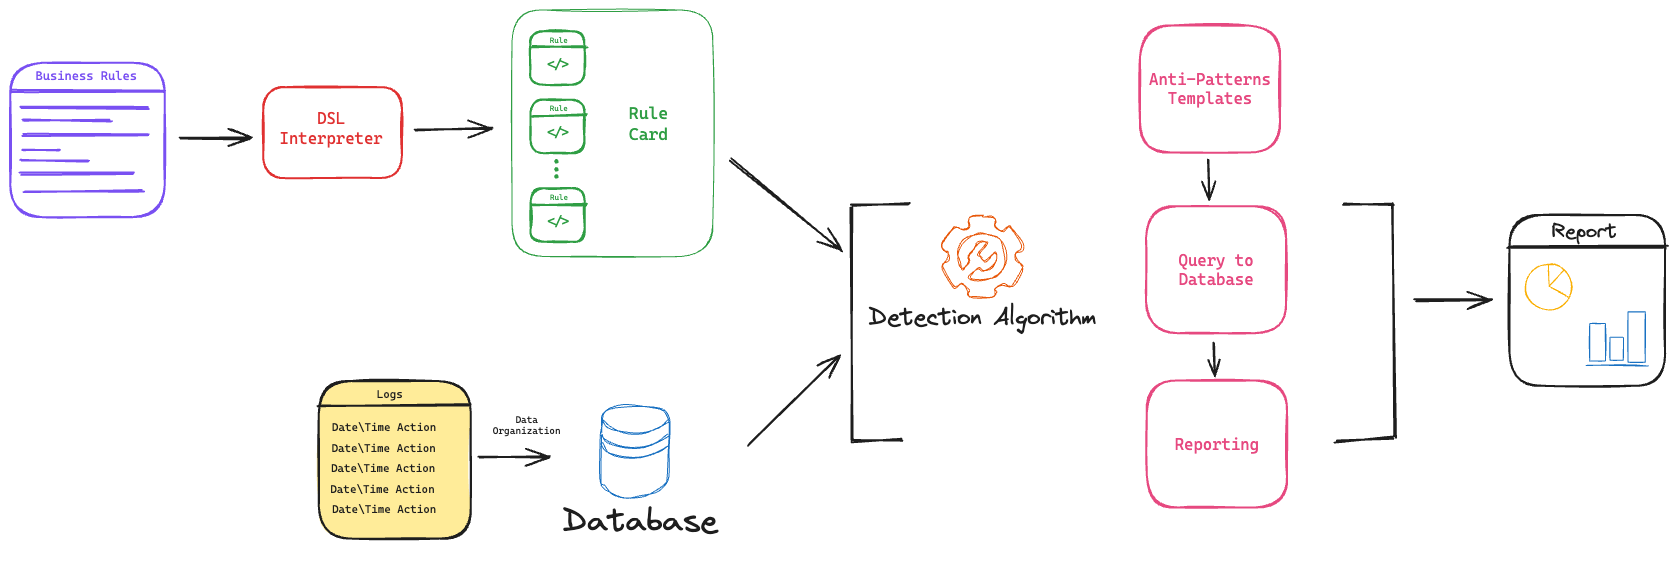
\includegraphics[scale=0.285]{basic_concept}
		\caption{The basic concept of work.}
		\label{fig:basic_concept}
	\end{figure}
	
	\subsubsection*{Component overview}
	
	\begin{enumerate}
		\item  \textbf{Business Rules:} Business rules \cite{business_rules} are one of 2 \textit{input parameters} of the system, which describes the rules at a high level for which the system may have performance vulnerabilities.
		\item \textbf{DSL Interpreter:} The DSL interpreter is one of the main and important components of the system, responsible for translating high-level business rules into rule cards described using a programming language. These rules define patterns that are considered indicators of potential anti-patterns in the system.
		\item  \textbf{Rule Cards:} Each rule card is an encapsulated set of instructions received from the DSL interpreter. They are intended to be applied directly to a database for query and analysis purposes.
		\item  \textbf{Logs and Databases:} The second \textit{input element} of the system is the information system logs. These logs are the most common ones, which contain information such as date, time, payload, response status and much more. This data is structured into a database to optimize data retrieval and query execution.
		\item  \textbf{Detection algorithm: }The heart of the system is the detection algorithm. This complex component uses a set of rule cards to scan a database, identifying and classifying anti-patterns based on predefined patterns.
		\item  \textbf{Anti-Pattrens Templates: }These patterns provide predefined, generic queries to identify deviations from normal patterns. They are essential for recognizing a variety of antipatterns, from simple anomalies to complex sequences that indicate deeper systemic problems.
		\item  \textbf{Query to Database: }This component is important because it searches the database for antipatterns.
		\item  \textbf{Reporting: }The last component of the system is the reporting module. It generates detailed reports and visualizations of detected antipatterns, presenting them in a format that is easy for users to interpret and understand.
	\end{enumerate}
	
	\subsubsection*{Data Flow}
	
	\hspace{5mm}Antipattern detection process begins with the DSL Interpreter translating business rules into rule cards(see section \ref{sec:dsl-translator}). These rule cards are then utilized by the Detection Algorithm to query the database for potential anti-patterns. Upon successful detection, the relevant data is compiled into reports that are both informative and easily digestible by the end-users.
	
	\subsubsection*{System Interaction}
	
	\hspace{5mm}Each component is designed to interact seamlessly with the others. For instance, the rule cards are created in a format that is directly executable by the Detection Algorithm, ensuring smooth data flow. The database is structured to support the complex queries generated by the Detection Algorithm, and the reporting tools are integrated to provide immediate feedback on detected anti-patterns.
	
	\subsubsection*{User Interface}
	
	\hspace{5mm}Design of the developed system includes a user-friendly interface that allows for the easy creation and modification of business rules, initiation of the detection process, and viewing of reports. It is designed to be intuitive, requiring minimal technical expertise to operate.
	
	\hspace{5mm}Architecture of the developed system facilitates efficient detection of anti-patterns in event logs, transforming complex business rules into actionable queries and insights. With a robust database, intelligent detection algorithm and user-centric reporting tools, the system can improve operational efficiency and help in proactive system management.
	
	\subsection{System Architecture}
	
	\hspace{5mm}Architecture\cite{system_arch} of the developed system for event logs is a comprehensive framework designed to facilitate the seamless translation of business rules into useful information for system optimization. The architecture is modular, with each component serving a specific function and working in harmony with the others. The next section will be devoted to the architectural principles of operation.
	
	\subsubsection*{Architectural principles}
	
	The project follows several key architectural principles:
	
	\begin{enumerate}
		\item  \textbf{Modularity: }Each component, such as the DSL interpreter, rule map, detection algorithm, and reporting module, is a separate unit that can be updated independently.
		\item \textbf{Scalability: }The system can handle growing volumes of event logs and complex queries without significant changes to its architecture.
		\item \textbf{Interoperability: }Each module is designed to work with different data sources and formats, ensuring compatibility with other systems.
	\end{enumerate}
	
	\subsubsection*{Technology Stack}
	
	\hspace{5mm}The system will use a combination of technologies such as SQL for database operation, an internal language such as Python \cite{python} for the detection algorithm, and an external environment. The technology stack will be discussed in more detail a little later, in the following sections.
	
	\hspace{5mm}System architecture is the design of a scalable and interoperable system. It is designed to effectively solve the problems of detecting anti-patterns in event logs and serve as a reliable tool for system analysts and administrators to maintain optimal system performance.
	
	\subsection{Methodology}
	
	\subsubsection{Service-Oriented Architecture}
	
	\hspace{5mm}Service-Oriented Architecture (SOA) is a design paradigm that organizes software components into reusable services, which can be accessed and combined to fulfill specific business functions \cite{soa}. In SOA, services are loosely coupled and interact through standard communication protocols, making it easier to integrate disparate systems and adapt to changing business requirements.
	
	\hspace*{5mm}SOA has gained popularity in big information systems due to several key factors. Firstly, its \textit{modular and reusable nature} allows organizations to break down complex functionalities into smaller, manageable components, facilitating easier development, maintenance, and evolution of large-scale systems. Secondly, SOA promotes \textit{seamless integration} by providing standardized interfaces for communication and interaction between disparate systems and technologies, enabling efficient data exchange and collaboration. Additionally, SOA architectures offer scalability and flexibility, allowing systems to scale horizontally to accommodate growing volumes of data and users while remaining agile and responsive to changing business needs. The capability for dynamic service discovery and composition further enhances agility by enabling real-time assembly of complex business processes from reusable services \cite{soa_2}. 
	
	\hspace*{5mm}The IS as the running example has an SOA architecture. CRS is a distributed software containing various client and server components. Fig.\ref{fig:dps} visualizes a more detailed structure of the product. As can be seen from the figure, at a high level we have business domains that implement separate business logic and do not interact with each other in any way. For example, there are business domains “booking” and “accounting". Processes are grouped into \textbf{process groups (PG)}, and services are grouped into \textbf{technical domains (TD)}. Returning to the previous example, there are PG and TD named “booking". Processes and services located in the same domain can interact with each other. But from outside, only process is available. That is, we get that processes in one domain can communicate with processes in another domain. Technically, all processes and services are implemented as interfaces and packages of a certain programming language. Each process and service sends and receives messages (corresponding to OperationName), and each specific message is logged as a separate trace in the log.
	
	\begin{figure}[h]
		\centering
		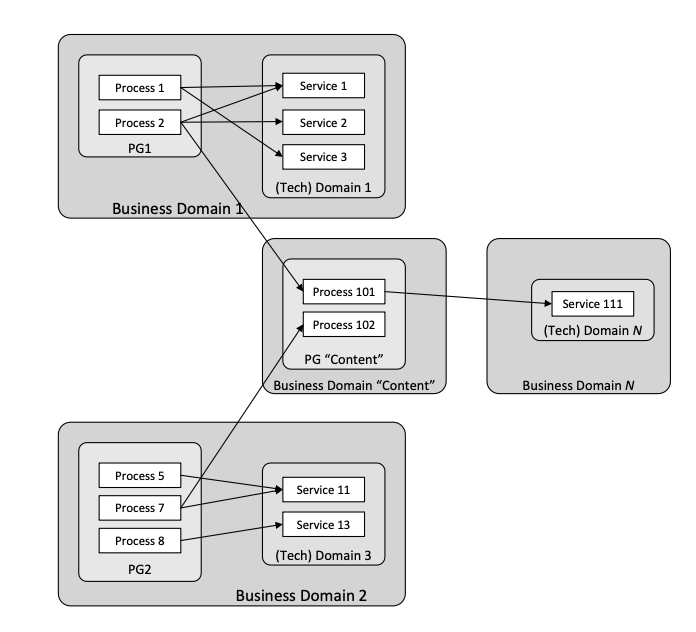
\includegraphics[scale=1]{DPS}
		\caption{“Domains-Processes-Services” architecture scheme.}
		\label{fig:dps}
	\end{figure}
	
	\hspace*{5mm}We have a set of logs that track the relationships between these processes and services and contain many different aspects of the data. By studying certain data representations, we can look at the system from different perspectives. Each particular view can represent some aspect of the system. We highlight aspects such as the control flow aspect, the data perspective, the organizational aspect and the infrastructural context.\newline
	\hspace*{5mm}In this section, we have considered what an information system based on SOA consists of. We looked at a basic example of how business domains, processes, and services interact with each other, and confirmed the fact that each interaction of these components is logged in an event log that we can use for analysis. More details about the contents of the logs will be mentioned in the next section.
	
	
	\subsubsection{Event Logs and Tools}
	
	\hspace*{5mm} Informally, event log is a chronologically ordered record of events occurring within a system or process, often used for troubleshooting and analysis purposes \cite{event_logs}. It can include various types of events, such as errors, warnings, information messages, and user actions. Each event is typically time stamped and includes additional information such as the source of the event and any relevant data associated with the event.
	
	\hspace*{5mm}Subsystems of CRS support the ability to track the interaction of all necessary processes and services. The initial call of any process, for example, made by an application with an extended client interface, is accompanied by the allocation of a special
	call identifier (\textit{also called InvID}). Both \textbf{processes (PR)} and \textbf{services (SV)} receive a \textbf{request message (RQ)} as input and the returned \textbf{response message (RS)} or \textbf{exception (SE)} as output. These messages are logged. At the log level, traces are recorded in XML format \cite{xml}. For the convenience of working with data, these events have been overwritten \cite{multi_perspective} in SQLite3 format \cite{sqlite3}. An example of such an event is given in the 
	Fig.\ref{fig:Interfaces1}.\\
	\hspace*{5mm}Each trace is included in a tracing event element that contains several sections describing the trace and including additional data that can be used for more in-depth analysis. For our first step, we are interested in the following data: \textbf{UnitName, PackName, InterfaceName}. Then we will also look at two very important fields. First, the timestamp of the event. In describing the second, we should mention that the trace event contains a payload specified in a form used by processes and services to exchange data with each other. The useful data is presented as a piece of data and can be used to analyze the model created using this log from a data perspective. 
	
	\begin{figure}
		\centering
		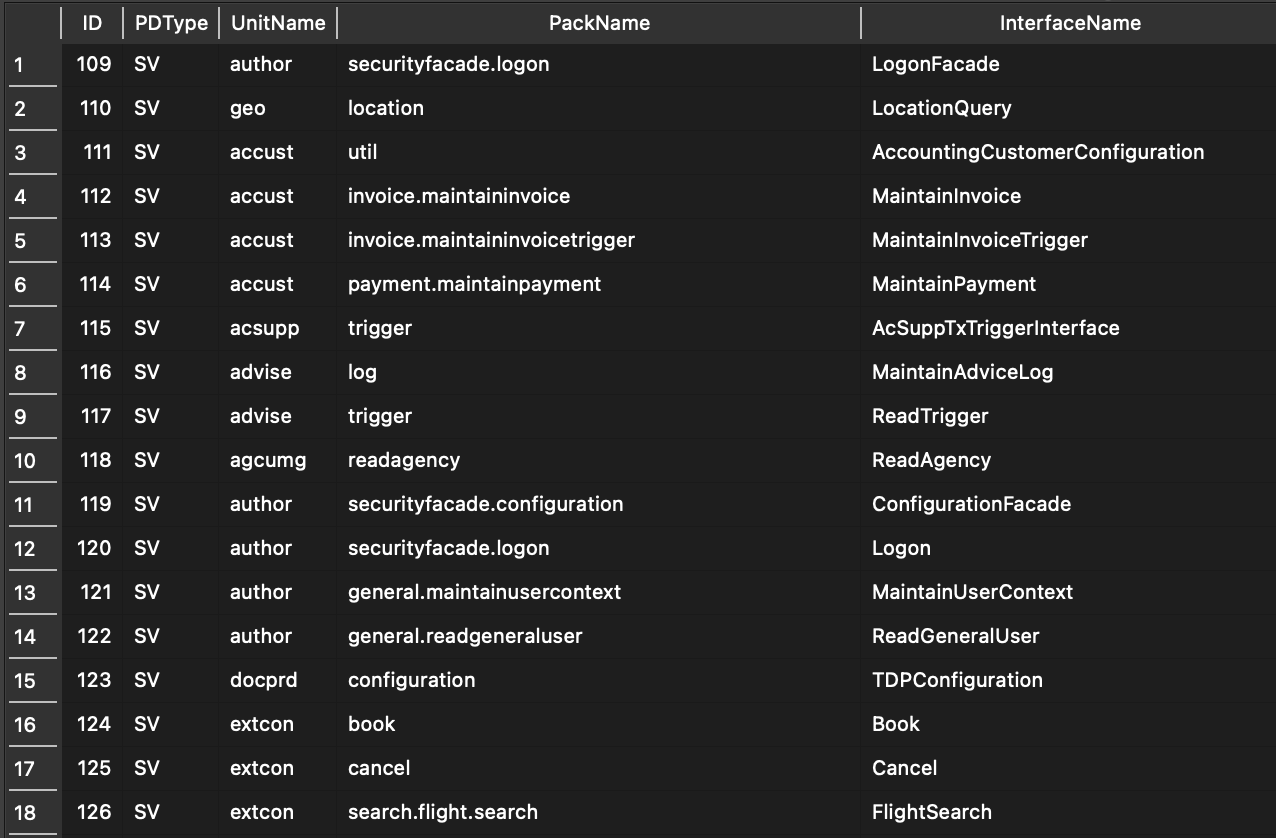
\includegraphics[scale=0.7]{Interfaces1}
		\caption{A table containing service interaction events.}
		\label{fig:Interfaces1}
	\end{figure}
	
	The TracingEvents table has a lot of interesting event data besides the payload. Below are all the fields that are contained in the table:
	
	\begin{itemize}
		\item \textbf{ID}: A unique identifier for the interface.
		\item \textbf{PDType}: The type of protocol or data format used.
		\item \textbf{UnitName}: The name of the unit associated with the interface.
		\item \textbf{PackName}: The package name associated with the interface.
		\item \textbf{InterfaceName}: The name of the interface.
		\item \textbf{ID}: A unique identifier for the event.
		\item \textbf{Interface\_ID}: The identifier linking the event to a specific interface.
		\item \textbf{OperationName}: The name of the operation or action associated with the event.
		\item \textbf{InvID}: The identifier associated with the event invocation.
		\item \textbf{InvNodeName}: The name of the node where the event invocation occurred.
		\item \textbf{InvIP}: The IP address associated with the event invocation.
		\item \textbf{TransContext\_ID}: The identifier linking the event to a transaction context.
		\item \textbf{AppServerContext\_ID}: The identifier linking the event to an application server context.
		\item \textbf{EventType}: The type of event, such as error, warning, or informational.
		\item \textbf{EventTimestamp}: The timestamp indicating when the event occurred.
		\item \textbf{PayloadSize}: The size of the payload associated with the event.
		\item \textbf{PayloadCRC32}: The cyclic redundancy check (CRC32) value for the payload.
		\item \textbf{EventSeqNum}: The sequence number of the event within the log.
		
	\end{itemize}
	
	\hspace*{5mm}One of the suggested anti-pattern search options is payload analysis among TracingEvents. That is, we will determine whether the size of her data and her hash amount change from call to call. You can also analyze the data for overloading services. When services interact, one service communicates with another until the first one receives the necessary information from the second. Sometimes, with incorrect software implementation of such interaction of services, calls are overloaded, which can have a bad effect on efficiency, and in the worst case, on its inactivity. To find such antipatterns in the logs, it is proposed to analyze the events for the number of calls.\\
	\hspace*{5mm}Such proposed solutions describe only the general concept of what the anti-pattern detection method is focused on and how it will work. In order for the proposed method to be universal and convenient for the end user, it is proposed to describe the rules by which anti-patterns will be searched in different information systems. For more information about what such rules are, how to create and describe them, see the next section
	
	\subsubsection{Rule-Based Systems and Domain-System Languages}
	
	\hspace*{5mm}In ISs, a rule-based system is a paradigm for encoding and executing logical rules to automate decision-making or problem-solving tasks \cite{rule}. These systems rely on a set of rules expressed in a formal language that defines conditions and actions. Each rule typically consists of an antecedent (condition) and a consequent (action), where the action is executed if the condition is satisfied. Rule-based systems are widely used in various domains, including business process management, expert systems, and workflow automation.\newline
	\hspace*{5mm}One of the key advantages of rule-based systems is their declarative nature, which separates the logic of the rules from the control flow of the program. This enables domain experts to define and modify rules without extensive programming knowledge, making rule-based systems accessible and adaptable to changing requirements. Additionally, rule-based systems facilitate transparency and traceability, as the logic governing decision-making is explicitly defined in human-readable form.\newline
	\hspace*{5mm}Domain-System languages (DSLs) are programming languages adapted to meet the specific needs and objectives of a specific domain or problem space \cite{dsl}. Unlike general-purpose programming languages, which are designed to be universal and applicable in various domains, DSLs are optimized to express concepts, abstractions, and operations within a specific domain.\newline
	\hspace*{5mm}In rule-based systems, DSLs are often used to define the syntax and semantics of rules depending on the domain. These DSLs provide a higher level of abstraction that closely aligns with users domain experience, allowing them to express rules in a natural and intuitive way. By encapsulating domain-specific concepts and designs, DSLs enhance the readability, maintainability, and usability of rule-based systems. DSLs in rule-based systems can offer specialized constructs to define conditions, actions, constraints, and relationships related to a specific subject area. These DSLs can also provide mechanisms for modularization, layout, and reuse of rule components, making it easier to develop and manage complex rule sets. \\
	\hspace*{5mm}In this section, we have gained a basic understanding of systems with rules, as well as about DSL, which is responsible for the implementation of such a system. The next section will describe the basic principles of the proposed method of detecting anti-patterns in logs.
	
	\subsubsection{DSL Interpreter}
	\label{sec:dsl-translator}
	
	\subsubsection*{Describing Rules Using DSL}
	
	\hspace*{5mm} Describing business rules usually does not require deep technical knowledge. It is enough to have an idea of the IS for which the rules will be described. Therefore, when compiling the syntax of the rules described using DSL, this important point was taken into account. 
	
	\hspace*{5mm}The syntax for this rule is shown in Listing \ref{lst:syntaх}. Each rule begins with the \textit{rule} keyword, followed by the rule name in quotation marks. The \textit{body} of the rule is described in curly braces and consists of a condition and an action. Conditions are specified with \textit{when} keyword. This block checks the conditions under which the rule should be activated. Actions are specified with \textit{then} keyword. This block defines the actions that must be performed if the conditions of the rule are met. In our case, this is the \textit{makeReport()} function, which generates a report.
	
	
	\begin{lstlisting}[language=Python, caption={Syntax of a rule described using DSL}, , label={lst:syntaх}]
rule "Long_Response_Time_Rule" {
  when
    ServiceA.RT > 100;
  then
    makeReport();
}
	\end{lstlisting}
	
\hspace*{5mm} When describing the conditions for executing a rule, you can use various arithmetic and logical operations (>, <, ==, !=). The \textit{left} operand must consist of a single expression separated by a dot. To the left of the dot, the name of the service, module, process or domain in which you want to search is described. To the right of the dot, you must indicate one specification (see section \ref{sec:specifications}). The right operand can be an nteger, float, string, or boolean value. Using the example shown in Listing \ref{lst:syntaх}, we specify a rule in which the response time of service A is more than 100 (milliseconds). The concept of a rules card using DSL represents several rules, an example of one of which we looked at above. Listing \ref{lst:syntaх2} shows an example of a rule card.

\hspace*{5mm}Currently, the system being developed can only generate a report. Therefore, each rule only has a \textit{makeReport()} event in the \textit{then} block. A report will not be generated for every rule. It will be done for the entire rule card.

\begin{lstlisting}[language=Python, caption={Syntax of a rule card using DSL}, , label={lst:syntaх2}]
rule "Long_Response_Time_Rule" {
  when
    ServiceA.RT > 100;
  then
    makeReport();
}

rule "High_Coupling_Rule" {
  when
    ServiceB.CPL = true;
  then
    makeReport();
}

rule "Low_Availability_Rule" {
  when
    ServiceC.A = false;
  then
    makeReport();
}
\end{lstlisting}
	
	\subsubsection*{Translating Rules into Rule Card}
	
	\hspace*{5mm}DSL Interpreter performs the function of converting rule cards described using DSL into a rule card in JSON, which will be used by the developed system to search for antipatterns in logs (see section \ref{sec:rule-card}). Why do you need such a card? Firstly, a card described using DSL is not convenient from a technical point of view. In order not to encounter consistency problems in the developed system, the rules will be described in JSON. On the card shown in Listing \ref{lst:syntaх2}, you can see fairly simple rules, which individually do not provide useful information for developers. That is, if the rule states that \textit{service A} has a \textit{long response time} and that \textit{service B} has \textit{high coupling}, then such a statement will not give us cause for alarm. The combination of such rules is precisely a sign of an \textit{antipattern}. That is, if we add the \textit{low availability} rule for service B to the rules described above, then we get a ready-made \textit{BottleneckService} antipattern. DSL Interpreter not only performs the conversion function from DSL to JSON, but also supplements the rules with any other suitable rules if they ultimately form a ready-made antipattern. Why did this role fall on Interpreter? The end user does not need to know about the concept of an antipattern, its types and what it consists of. To make the user’s life easier, the process of initialization and generation of a ready-made rules card, which formally will contain information about the antipattern, will be performed in DSL Interpreter.
	
	\subsection{Algorithm for Translating a Rule Card into an SQL Query}
	
	This subsection outlines an algorithm designed to translate a rule card, provided in JSON format, into an SQL query. The purpose of this algorithm is to generate an SQL query that identifies specific anti-patterns in log data, based on the rules defined within the rule card.
	
	\subsubsection*{Input and Output}
	\hspace*{5mm} The input to the algorithm is a JSON object representing the rule card. An example is provided in section \ref{sec:examples}. The output of the algorithm is an SQL query that searches for the anti-pattern specified by the rule card. For the example input(Fig. \ref{fig:nobody_home}), the output would be like in Listing \ref{lst:sql1}. 
	
\begin{lstlisting}[language=SQL, caption={SQL Query for NobodyHome Antipattern}, , label={lst:sql1}]
SELECT OperationName, EventType, count(*) as nir, avg(PayloadSize) as nmi 
from FullData3
WHERE EventType == "RS"
Group by OperationName,  EventType
HAVING nir <= ordi_value AND nmi > ordi_value
ORDER by nir, nmi DESC
\end{lstlisting}

	\hspace*{5mm} The IS being developed contains a list of antipatterns that the system can find from logs. Taking into account the fact that different information systems, which in the future will implement the product being developed, have different log structures. In order for the system to function correctly and find antipatterns in the logs, before the first launch of the system, it is necessary to initialize the names of key parameters in the logs. For example, the parameter storing the payload can be called \textit{Payload}, \textit{PayloadSize} or \textit{Volume}. To avoid confusion, the end user must configure the system being developed in advance.
	
	\subsubsection*{Algorithm Overview}
	The algorithm consists of the following steps:
	
	\begin{enumerate}
		\item \textbf{Parse the JSON Input:}
		\begin{itemize}
			\item Extract the primary rule card name.
			\item Extract the list of rules.
		\end{itemize}
		\item \textbf{Initialize SQL Components:}
		\begin{itemize}
			\item Initialize the \texttt{SELECT} clause to specify the columns to be selected.
			\item Initialize the \texttt{FROM} clause to specify the table involved.
			\item Initialize the \texttt{WHERE} clause to specify the conditions based on the rules.
		\end{itemize}
		\item \textbf{Generate Conditions Based on Rules:}
		\begin{itemize}
			\item For each rule, generate the corresponding SQL condition based on the rule's \texttt{metric\_id} and \texttt{ordi\_value}.
			\item Handle complex conditions where multiple rules are combined using logical operators (e.g., \texttt{INTER} for intersection).
		\end{itemize}
		\item \textbf{Combine Conditions:}
		\begin{itemize}
			\item Combine individual rule conditions using appropriate logical operators.
		\end{itemize}
		\item \textbf{Construct the SQL Query:}
		\begin{itemize}
			\item Combine all the SQL components into a single SQL query.
		\end{itemize}
	\end{enumerate}
	
	\hspace*{5mm} This algorithm ensures that the SQL query accurately reflects the conditions specified in the rule card, enabling effective identification of anti-patterns in the logs.
	
	\subsection{Workflow of the Development System}
	
	\hspace*{5mm}This section will describe the basic principle of the method proposed in this paper for detecting anti-patterns in event logs.  Earlier, we learned what an event log is and what logs it consists of. We looked at an example of data from the railway ticket booking system. We also figured out what a rule-based system is, and what tools are needed for this. Fig.\ref{fig:scheme} shows the general scheme of the system, which was obtained on the basis of all the knowledge obtained just above.
	
	\begin{figure}[h]
		\centering
		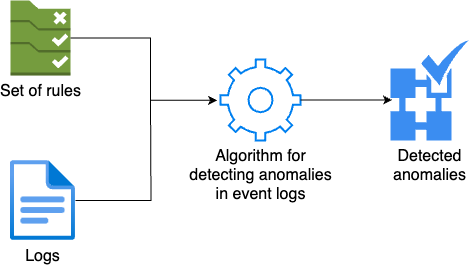
\includegraphics[scale=0.7]{scheme}
		\caption{The basic principle of the system operation.}
		\label{fig:scheme}
	\end{figure}
	
	\hspace*{5mm}The operation of the system can be described in more detail as follows: a set of rules and logs is provided as input to the antipattern detection method. The rules are described using a DSL. The number of rules is limited. Logs need to be transferred and grouped into DB-based format such as \textit{SQ3EventLog}. These parameters are then passed as input to the antipattern detection method. A method based on these rules executes a complex SQL query against a database. Next, the database is analyzed for the content of antipatterns. At the end of the search based on the results obtained by the method, the system issues a report on the work done, which will describe in detail the search results for each rule. \\
	\hspace*{5mm}This system is implemented as a framework in Python \cite{python}. This choice of programming language is associated with the convenient and flexible ability to integrate into various information systems. The next section will be devoted to the software implementation of the product being developed.
	
	\clearpage
	\newpage
	
	
	\section{System Implementation}
	
	\subsection{Tools and Technologies}
	
		\hspace*{5mm}The development of the anti-pattern detection system was underpinned by a selection of technologies chosen for their reliability, flexibility, and performance. This section outlines the technologies employed and the rationale for their use.
		
		\subsubsection*{JSON}
		
		\hspace*{5mm} JSON is used to describe the rules and metrics of antipatterns. This provides a number of advantages over using a domain-specific language (DSL), such as the one used by Francis Palma and co-authors.:
		
			\begin{itemize}
			\item \textbf{Accessibility and Familiarity:} JSON is widely used and understood in the software development community due to its simplicity and compatibility with various data formats. It's easier for developers who are already familiar with JSON to adopt and integrate it into existing systems without the need to learn a new syntax, as would be required with a DSL.
			\item \textbf{Interoperability:} JSON is a language-independent data format, making it highly interoperable across different platforms and programming environments. This flexibility allows our rule-based detection system to be more easily integrated with other applications and systems, which might not be the case with a specialized DSL.
			\item \textbf{Ease of Use:} JSON's structure is both human-readable and machine-parsable, facilitating easier debugging, testing, and maintenance of the rule definitions. Developers can quickly understand and modify the JSON-described rules without navigating the complexities of a more esoteric DSL syntax.
			\item \textbf{Tooling and Support:} There is robust tooling available for JSON processing, including parsers and libraries across all major programming languages, which can significantly reduce the time and effort required to implement and manage the system.
			\item \textbf{Scalability:} JSON's lightweight nature makes it well-suited for applications that require high performance and scalability. Managing and updating JSON files is generally less resource-intensive compared to processing DSLs, which can sometimes involve more complex parsing mechanisms.
		\end{itemize}
		
		\subsubsection*{Python}
		
		At the heart of our system's DSL interpreter and detection algorithm lies Python, a language chosen for several key reasons:
		
		\begin{itemize}
			\item \textbf{Versatility:} Python's extensive range of libraries and frameworks enables rapid development of complex applications.
			\item \textbf{Readability:} The language's clear syntax promotes a maintainable and comprehensible codebase, essential for the project's long-term viability.
			\item \textbf{Community Support:} A robust community and extensive documentation ensure that solutions for potential issues are easily accessible.
			\item \textbf{Integration Capabilities:} Python's ability to work seamlessly with other technologies and services made it an optimal choice for a system requiring interaction with a variety of components and data formats.
		\end{itemize}
		
		\subsubsection*{SQL}
		
		\hspace*{5mm}SQL was selected for database querying due to its powerful data retrieval and manipulation capabilities, being particularly well-suited for managing structured data in relational databases. The system's need for complex query execution and large-volume data handling rendered SQL an essential component of the technology stack.
		
		\begin{itemize}
			\item \textbf{Efficiency:} SQL's data manipulation and querying proficiency allows for rapid searches across extensive datasets, pivotal for real-time anti-pattern detection.
			\item \textbf{Universality:} As a standard that is widely adopted, SQL ensures database operations are compatible with various database management systems.
			\item \textbf{Scalability:} The scalability of SQL databases aligns with the requirement to handle an expanding volume of event log data.
		\end{itemize}
		
		\subsection*{Integration and Deployment}
		
		\hspace*{5mm}The integration of the Python logic with SQL querying was facilitated through a dedicated interface, ensuring seamless communication between the application layer and the database. The architecture was designed to support deployment in diverse environments, accommodating both on-premises and cloud-based infrastructures.
		
		\hspace*{5mm}The synergistic use of Python and SQL forms a solid foundation for the anti-pattern detection system. The flexibility and user-friendliness of Python, combined with the robust data handling capabilities of SQL, result in a powerful yet adaptable system, ready to meet the dynamic requirements of the European Travel Computer Reservation System (CRS).


	\subsection{Antipatterns and Specifications}
	\label{sec:specifications}
	
	\hspace*{5mm} In the context of work, antipatterns refer to common, repetitive incorrect practices or design flaws in the architecture of service-based systems that can lead to reduced performance, reduced usability, increased complexity, or other negative consequences. In fact, they represent "bad solutions" to common problems where better solutions are known to exist. In this work, antipatterns generally accepted by various scientific communities \cite{doc} were used, such as:
	
	\begin{enumerate}
		\item \textit{Bottleneck Service} is a service that is highly used by other services or clients. It has a \textbf{high incoming and outgoing coupling}. Its \textbf{response time} can be \textbf{high} because it may be used by too many external clients, for which clients may need to wait to get access to the service. Moreover, its \textbf{availability} may also be low due to the traffic.
		\item \textit{Chatty Service} corresponds to a set of services that exchange a lot of \textbf{small data of primitive types}, usually with a \textbf{Data Service} antipattern. The Chatty Service is also characterized by a \textbf{high number of method invocations}. Chatty Services chat a lot with each other \cite{book_1}.
		\item \textit{ Data Service} in Object-Oriented \cite{book_2} systems, corresponds to a service that contains \textbf{mainly accessor methods}, i.e., getters and setters. In the distributed applications, there can be some services that may only perform some simple information retrieval or data access to such services. Data Services contain usually \textbf{accessor methods} with \textbf{small parameters of primitive types}. Such service has a \textbf{high} data \textbf{cohesion}.
		\item \textit{Duplicated Service}, introduced by IBM, corresponds to a set of \textbf{highly similar services}. Because services are implemented multiple times as a result of the silo approach, there may have \textbf{common} or \textbf{identical methods} with the \textbf{same names and–or parameters} \cite{duplicated_service}.
		\item \textit{LostData Service} antipattern appears when data essential for the completion of business processes is misplaced or lost during transitions between services. It typically indicates poor data handling or integration practices within the system.
		\item \textit{Multi Service} also known as \textit{God Object} corresponds to a service that implements a \textbf{multitude of methods} related to different business and technical abstractions. This service aggregates too many methods into a single service, such a service is not easily reusable because of the \textbf{low cohesion} of its methods and is often \textbf{unavailable} to end-users because of it is \textbf{overloaded}, which may also induce a \textbf{high response} time \cite{book_1}.
		\item \textit{Nobody Home} corresponds to a service, defined but actually never used by clients. Thus, the methods from this service are \textbf{never invoked}, even though it may be \textbf{coupled} to other services. Yet, it still requires deployment and management, despite of its non-usage \cite{nobody_home}.
		\item \textit{Service Chain} \cite{book_2} in Object-Oriented systems corresponds to a \textbf{chain of services}. The Service Chain appears when clients request consecutive service invocations to fulfill their goals. This kind of \textbf{dependency} chain reflects the subsequent \textbf{invocation} of services.
		\item \textit{The Knot} is a set of \textbf{very low cohesive} services, which are \textbf{tightly coupled}. These services are thus less reusable. Due to this complex architecture, the availability of these services may be \textbf{low}, and their \textbf{response time high} \cite{book_3}.
		\item \textit{Tiny Service} is a small service with \textbf{few methods}, which only implements part of an abstraction. Such service often requires \textbf{several coupled} services to be used together, resulting in higher development complexity and \textbf{reduced usability}. In the extreme case, a Tiny Service will be limited to \textbf{one method}, resulting in many services that implement an overall set of requirements \cite{book_1}.
	\end{enumerate}
	
	\hspace*{5mm} The antipatterns described above are quite complex, especially for the end user. To simplify this task, specifications (metrics) were introduced \cite{soda}, through which these anti patterns will be described. The metric suite encompasses both static and dynamic metrics. The static metric suite includes (but is not limited to) the following metrics: number of methods declared (NMD), number of incoming references (NIR), number of outgoing references (NOR), coupling (CPL), cohesion (COH), average number of parameters in methods (ANP), average number of primitive type parameters (ANPT), average number of accessor methods (ANAM), and average number of identical methods (ANIM). The dynamic metric suite contains: number of method invocations (RMI), number of transitive methods invoked (NTMI), response time (RT), and availability (A). As a novelty for the current work, new indicators were added: the number of encapsulated services (NS), the total number of parameters (NP), the number of interfaces (NI) and the number of auxiliary methods (NUM), the payload volume (PLD).
	
	\hspace*{5mm} In this section, the basic antipatterns and their specifications have been identified, which will be used to find vulnerabilities in the system based on logs. The next section will be devoted to the rules card, namely to its definition, to its composition.
	
	\subsection{Rule Cards}
	\label{sec:rule-card}
	
	\subsubsection{Grammar}
	
	\hspace*{5mm} The rule card is the output of the DSL Interpreter, which converted and expanded the rule card described using the DSL into JSON. In developing the principle of drawing up such a card, it was important to take this point into account, because it should be easy to compose, understand, and read, not only by the author of the card, but also by any other third-party person. Based on existing work \cite{doc}, where the rules were described using a Backus-Naur Form, for development and support, which requires a lot of resources and effort, it was decided to simplify the task and define the card using JSON. The advantages of using JSON were defined earlier in the Tool and Technologies section. 

\iffalse
\begin{verbatim}
		1 rule_card      = rule card name
		2 rules          = array of rules [rule]
		3 rule           = name metric | relationship | operator 
		4 operator       = INTER | UNION | DIFF | INCL | NEG
		5 metric         = id_metric ordi_value | id_metric comparator num_value
		6 id_metric      = NMI | NRI | NOR | CPL | COH | ANP | ANPT | RT | A | PLD
		7 ordi_value     = very_high | high | medium | low | very_low
		8 comparator     = equal | less | less_equal | greater | greater_equal
		9 relationship   = relationType FROM ruleName cardinality TO ruleName cardinality
		10 relationType  = assoc | compos
		11 cardinality   = one | many | one_or_many | num_value NUMBER_OR_MANY
		12 rule_card, ruleName is String
		13 num_value is Double
\end{verbatim}
\fi


	\hspace*{5mm} The Fig.\ref{fig:rules} shows the structure of the description of the rules card. The syntax of the rules card is quite easy to understand. It consists of 2 parameters: the name of the \textit{rule\_card} card and the \textit{rules} array itself. Each rule consists of a \textit{name} and one \textit{specification}. The specification can be a metric described in the \textit{Antipatterns} section. A relationship or an operator can also serve as a specification. If we consider the specification of the metric in more detail, we can see that it comes in 2 types: with an indication of \textit{ordi\_value} and with an indication of comparator\textit{ num\_value}. \textit{ordi\_value }and \textit{num\_value} show how much the metric has a strong infusion on the process. That is, for example, if we have the RT high specification, it means that the response time of the service is high, or if we have the PLD equal 0 specification, it means that the useful load transmitted by the service is zero.
	
	\begin{figure}[h]
		\centering
		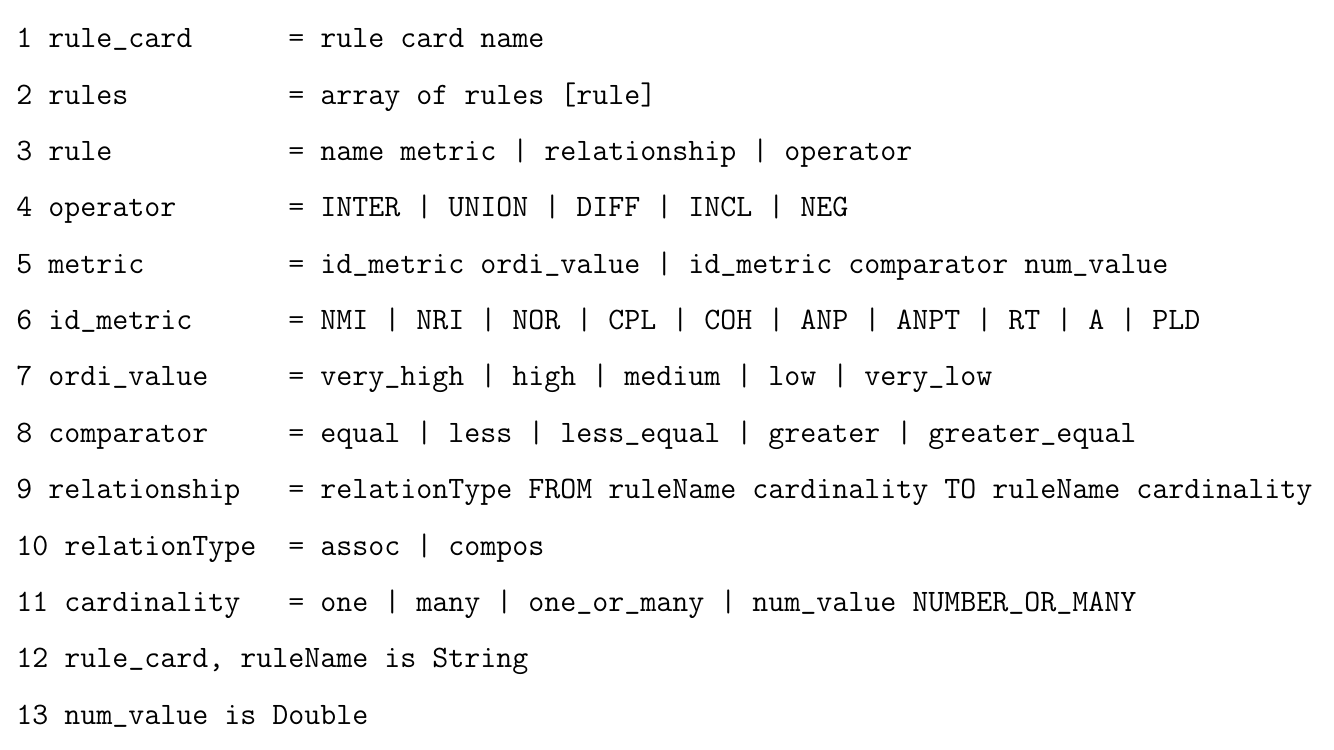
\includegraphics[scale=0.8]{rules}
		\caption{Grammar of Rule Cards}
		\label{fig:rules}
	\end{figure}
	
	The following Figures \ref{fig:bottleneck}, \ref{fig:chatty}, \ref{fig:duplicate}, \ref{fig:multiservice}, \ref{fig:nobody_home}  will provide examples of anti-pattern descriptions using the rules card. 
	
	\subsubsection{Examples}
	\label{sec:examples}
	
	\begin{figure}[h]
		\centering
		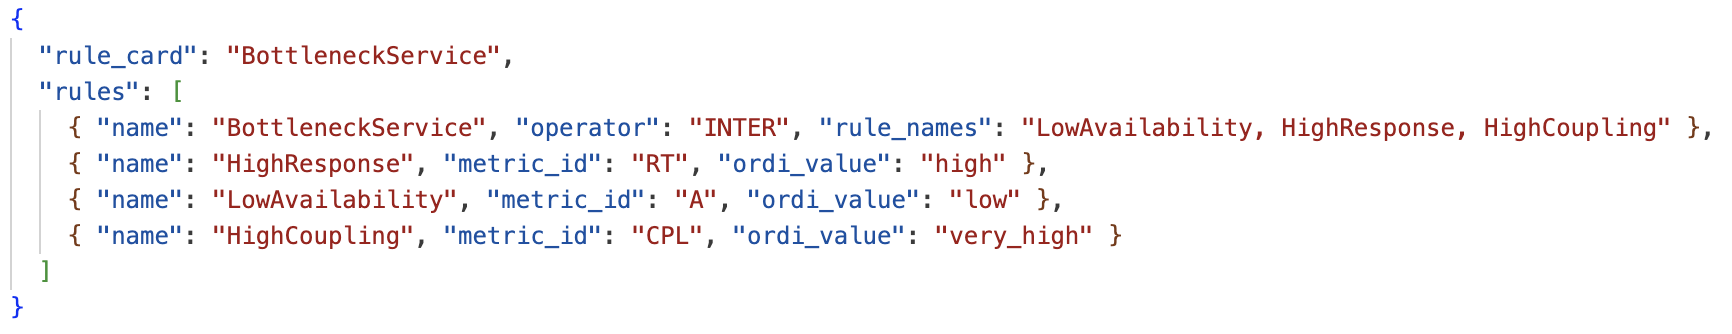
\includegraphics[scale=0.6]{bottleneck}
		\caption{"Bottleneck Service" Rule Card}
		\label{fig:bottleneck}
	\end{figure}

	\begin{figure}[h]
		\centering
		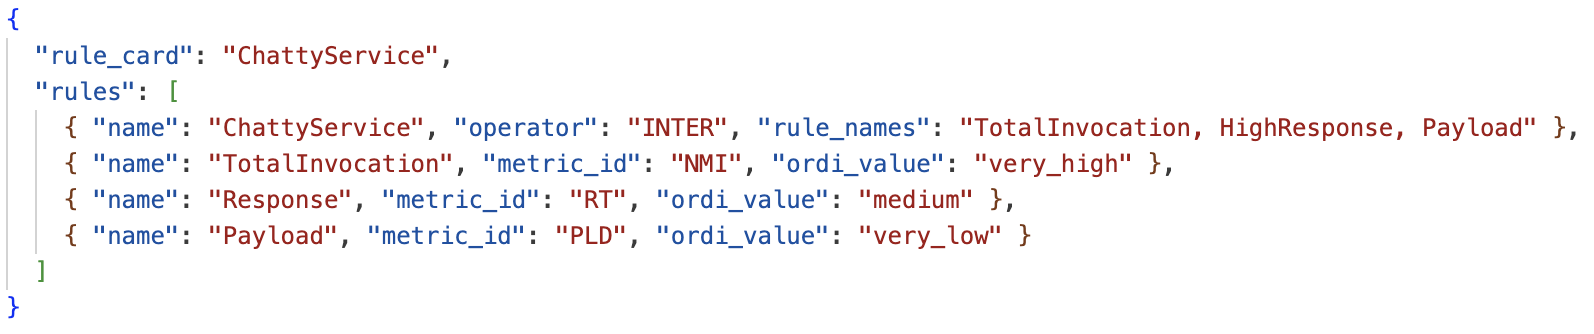
\includegraphics[scale=0.6]{chatty}
		\caption{"Chatty Service" Rule Card}
		\label{fig:chatty}
	\end{figure}	

	\begin{figure}[h]
		\centering
		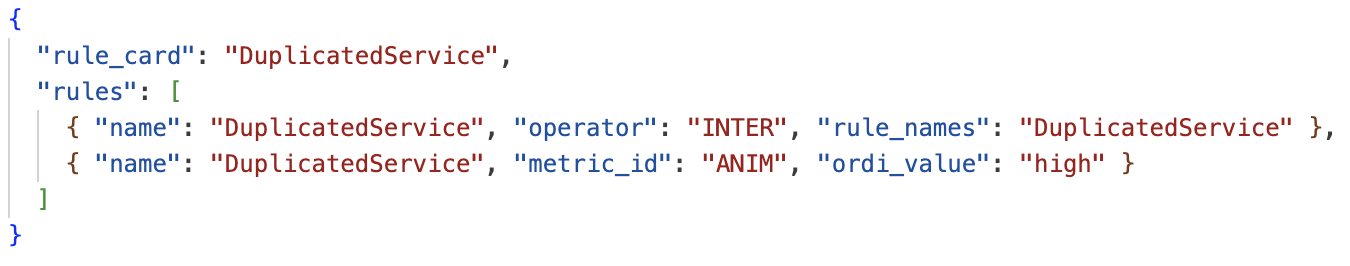
\includegraphics[scale=0.7]{duplicate}
		\caption{"Duplicate Service" Rule Card}
		\label{fig:duplicate}
	\end{figure}
	
	\clearpage		
	
	\begin{figure}[h]
		\centering
		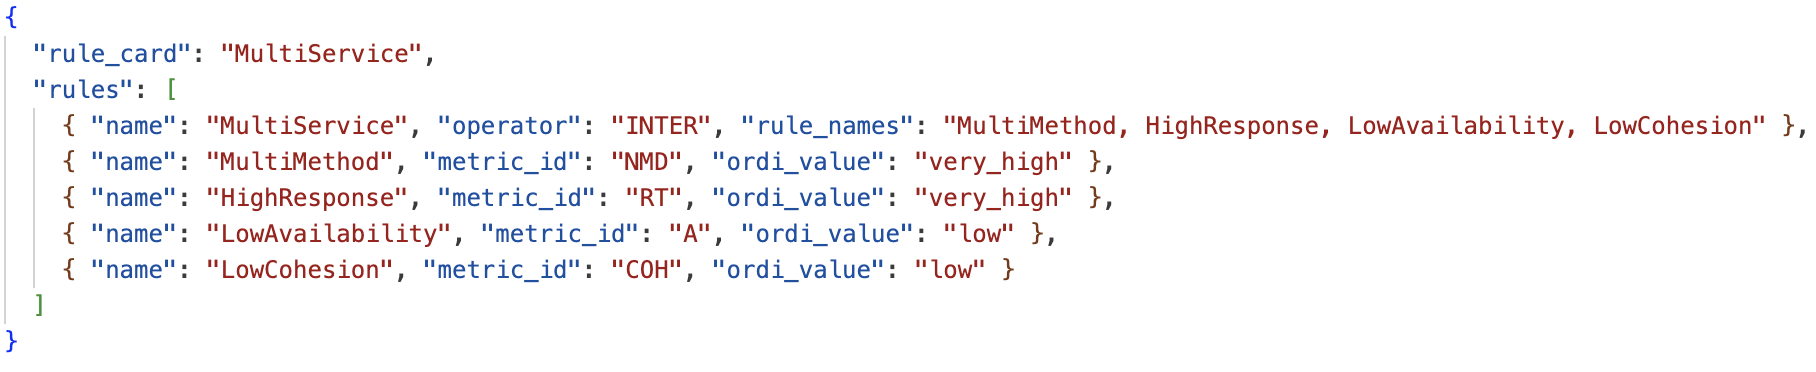
\includegraphics[scale=0.6]{multiservice}
		\caption{"Multi Service" Rule Card}
		\label{fig:multiservice}
	\end{figure}
	
	\begin{figure}[h]
		\centering
		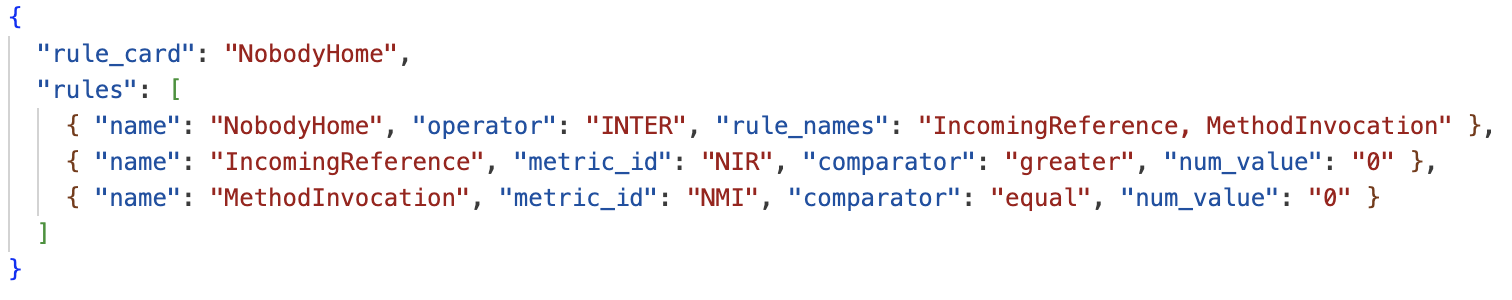
\includegraphics[scale=0.6]{nobody_home}
		\caption{"Nobody Home Service" Rule Card}
		\label{fig:nobody_home}
	\end{figure}
	
	\hspace*{5mm} Let's look at the rule card for the \textit{Bottleneck} antipattern that shown on Fig.\ref{fig:bottleneck}. The array of rules consists of 4 elements. The first rule is the \textit{operator} specification. The example indicates that filtering will be done using the intersection of the listed rules \textit{LowAvailability, HighResponse, HighCoupling}. The remaining 3 elements of the array are defined using the \textit{mertic\_id} specification. In this example, it is indicated that the Bottleneck antipattern is characterized by high response time, low availability and very high coupling of internal services. 
	
	\hspace*{5mm} As another example, consider the \textit{Nobody Home} antipattern shown in Fig.\ref{fig:nobody_home}. This antipattern is described using 3 rules: the main 2 rules are described using the \textit{metric\_id} and comparator specifications. In this example, we have that it is typical for this antipattern that the \textit{IncomingReference} number will be greater than zero and the \textit{MethodInvocation} number will be zero. The third rule shows us that it is necessary to \textit{intersect} the results of these 2 rules in order to get the final result. 
	
	\hspace*{5mm} In this section, the grammar of the rules cards was described, its structure and several examples of such cards were analyzed. By following this grammar, you can define a rule card for many other anti-patterns. The next section will be devoted to the implementation of the finished product. All its constituent components will be considered.
	
	\subsection{Implementation Structure}
	
	 \subsubsection{Overview}
	
	 \begin{figure}[h]
		\centering
		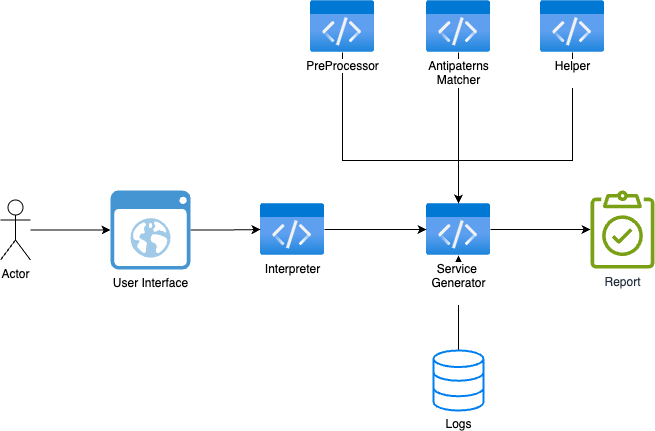
\includegraphics[scale=0.6]{scheme2}
		\caption{Implementation Structure}
		\label{fig:scheme2}
	\end{figure}
	
	 \hspace*{5mm} Fig.\ref{fig:scheme2} shows the implementation structure of the developed antipattern detection method. To make it convenient for the user to use this tool, a User Interface was implemented in which the user can select predefined rule cards with antipatterns. In more detail, what other components the system consists of is described below:
	 
	 \begin{itemize}
	 	\item \textbf{Actor:} This is a user initiating the process by uploading a rule card and event logs of an information system to trigger events that require analysis.
	 	\item \textbf{User Interface (UI):} This component serves as an interface through which the performer interacts with the system. This is where the user uploads the JSON file with the rules card and the IS logs. The selected files are then sent to the interpreter for further analysis.
	 	\item \textbf{Interpreter:} This module processes input data from the user interface, interpreting commands and data. It acts as an intermediary between the user interface and subsequent processing steps, ensuring proper formatting and forwarding of input data. Its main purpose is to \textit{validate} the rules card. She checks that the card was written without errors, that all the specifications specified in the card exist. At the exit of the interpreter, we get a validated card that will be used in the main module of the \textit{Service Generator}.
	 	\item \textbf{Helper:} This is one of the three auxiliary modules of the system. The main purpose of this module is to identify the antipattern according to the specifications verified by the interpreter.
	 	\item \textbf{Antipattern Matcher:} This module is responsible for \textit{generating} an SQL query to search for an antipattern in the event database. The SQL query is formed from the results obtained from the Helper module. \textit{Antipattern Matcher} does not interact directly with the \textit{Helper} module, so as not to overload the module itself and making it easily changeable and integrated into other areas of the system.
	 	\item \textbf{Preprocessor:} The preprocessor module performs the initial processing of data, preparing it for more detailed analysis. This includes cleaning up the data, structuring it, or extracting the necessary elements.
	 	\item \textbf{Service Generator:} This module is the heart of the system being developed, as it implements the main method of exposing antipatters. This module imports 3 auxiliary modules: \textit{Helper, AntipatternsMatcher, PrePocessor}. This module, after receiving a \textit{validated} rule card using Helper and AntipatternsMatcher, has a ready-made SQL query database of events of a certain IS. Then, using this SQL, a query will be executed in the database. The results will be preprocessed using the PreProcessor module. The final results will be recorded in a report that will be available to the user in the format \textit{.xlsx}.
	 	\item \textbf{Logs:} This database collects logs from various stages of the process of an information system. It stores data that will be used for further analysis, search and debugging.
	 	\item \textbf{Report:} The end result of the process is a report created based on data received from the Service Generator module. This report contains a summary table with detailed information about the detected antipatterns, broken down by the entered specifications. More information about this report will be described in the section \ref{sec:res}.
	 \end{itemize}
	 
	 \subsubsection{UI}
	 
	  \hspace*{5mm} As described earlier, the UI module is the connecting link between the user and the system being developed. And it was important when designing this interface to make it as simple and understandable as possible for the user. The Fig.\ref{fig:ui1} shows the main screen of the system. There are 3 buttons on it: A button for selecting a JSON file with a rule card, a button for selecting logs/databases, and a button for launching an anti-pattern detection method based on these input parameters. This button becomes available only when 2 input files are selected. There is also a file load indicator on the screen. It indicates whether the desired file has been selected. Fig.\ref{fig:ui2} shows how the screen should look when the user has done everything right to start the system.
	  
	  \begin{figure}[h]
	  	\centering
	  	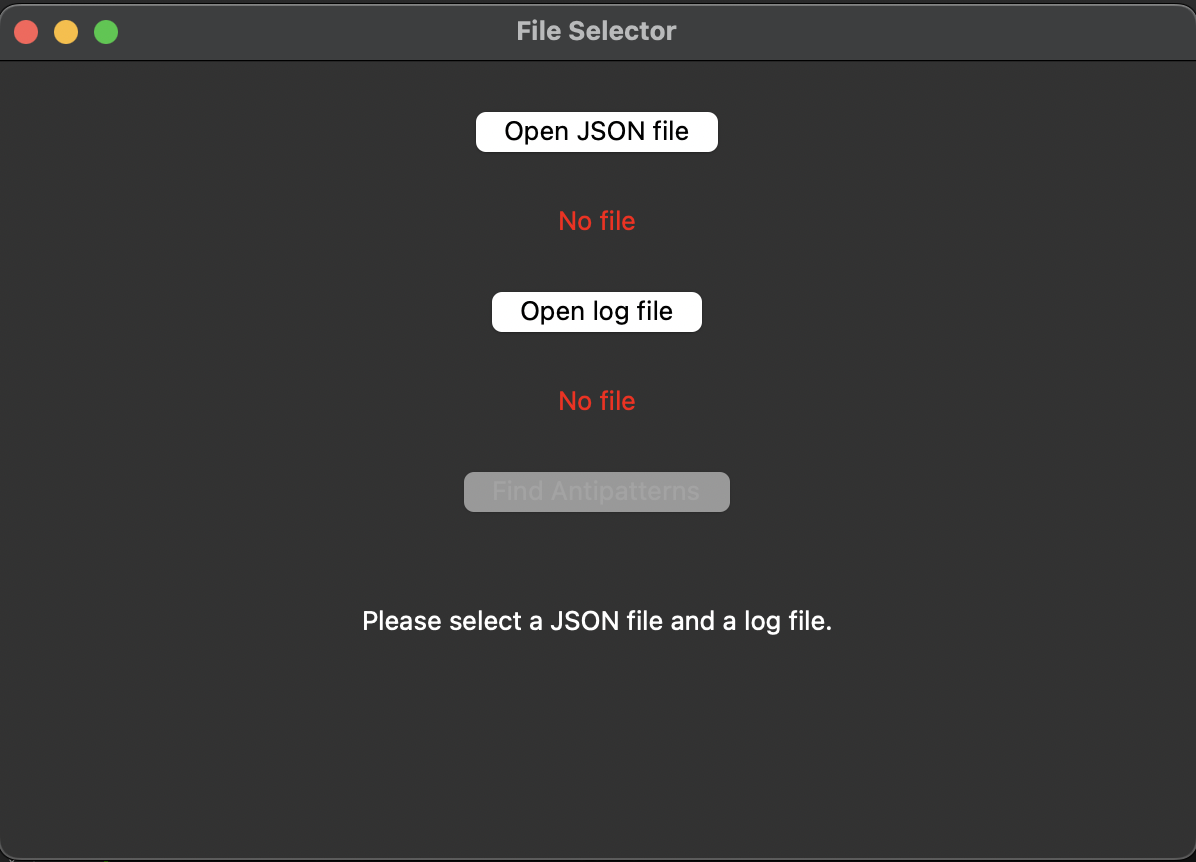
\includegraphics[scale=0.6]{ui1}
	  	\caption{Initial state of UI}
	  	\label{fig:ui1}
	  \end{figure}
	  
	  Fig.\ref{fig:ui3} shows the notification that should appear when the system completes successfully. After this notification appears, generated system report will automatically opened to user. Example of this report is shown on Fig.\ref{fig:res1}. The generated report will be saved in the root folder with the source code in \textit{.xlsx} format. This type of file was chosen for convenient and detailed viewing of all names of operations, services, modules for which the original business rule was executed. That is, the items on the list should be reviewed by IS engineers to revise their system architecture. Each time the system starts, a new file will be generated with the name specified in the rules card. If you do not change the name of the card, but only its content, then the old generated report will be lost. Subsection \ref{sec:res} describes in more detail how to analyze the results obtained in the report.
	  
	    \begin{figure}[h]
	  	\centering
	  	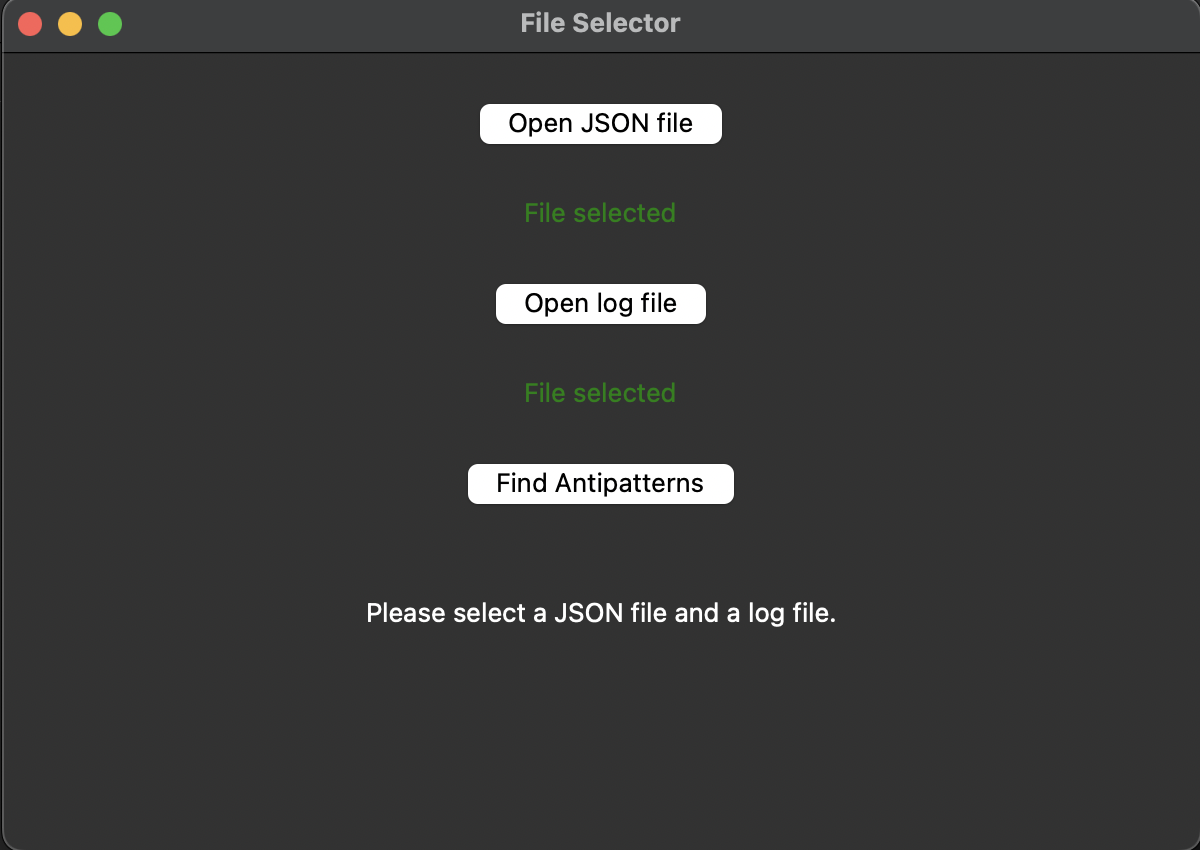
\includegraphics[scale=0.6]{ui2}
	  	\caption{The state of the UI when everything is loaded correctly}
	  	\label{fig:ui2}
	  \end{figure}

	\begin{figure}[h]
		\centering
		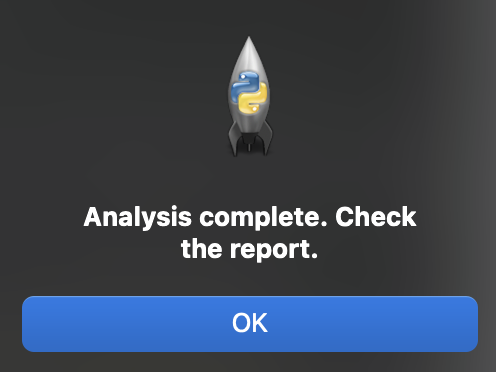
\includegraphics[scale=0.6]{ui3}
		\caption{Receiving notification when system finishes successfully}
		\label{fig:ui3}
	\end{figure}

	\begin{figure}[h]
		\centering
		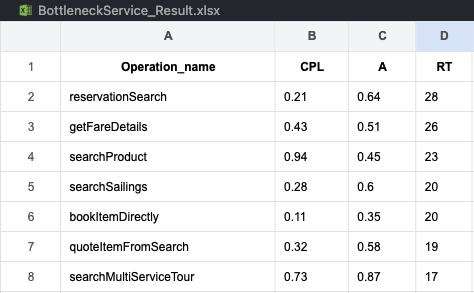
\includegraphics[scale=0.6]{res1}
		\caption{Generated report}
		\label{fig:res1}
	\end{figure}	
	
	
	\subsubsection{Service Generator}
	
	\hspace*{5mm} This module is the main one, so let's look at it in more detail. To configure this parameter, we will need: a name, an operator, an array of rules and logs/database. After initialization, we run the \textbf{main()} method, which has the structure presented in the Listing \ref{lst:service}. Listing \ref{lst:detect} and \ref{lst:sql} present methods for obtaining an antipattern based on rules and their specifications and a method for executing a query in the database.
	
	\begin{lstlisting}[language=Python, caption={Main method in Service Generator}, , label={lst:service}]
	def main(self):
	  antipattern = self.detect_antipattern_based_on_rules()
	  query_result = self.execute_query(antipattern)
	  self.result_process(query_result, antipattern)
	\end{lstlisting}

	\begin{lstlisting}[language=Python, caption={Method for detecting antipattern based on rules}, , label={lst:detect}]
	def detect_antipattern_based_on_rules(self):
	  antipattern = ''
	  metrics_id = list(self.rules.keys())
	  for item in Antipattern:
	    if set(metrics_id) == set(item.value):
		  antipattern = item.name
		  break
	  return antipattern
	\end{lstlisting}


	\begin{lstlisting}[language=Python, caption={Method for executing antipattern based SQL query}, , label={lst:sql}]
	def execute_query(self, antipattern, logs):
	  conn = sqlite3.connect(logs)
	  cursor = conn.cursor()
	  query = AntipatternsMatcher.sql_queries[antipattern]
	  cursor.execute(query)
	  results = cursor.fetchall()
	  conn.close()
	  return results
	\end{lstlisting}	
	
	\hspace*{5mm}The next and final result will be devoted to the results obtained. We will look at the format in which the system issues the report, look at its contents, analyze a couple of examples and draw conclusions based on the results obtained.
	
	\subsection{Results Analysis}
	\label{sec:res}
	
	\hspace*{5mm} In this subsection, we analyze the results of the rule-based antipattern detection method applied to various services. We focus on the detection of Bottleneck Service, Chatty Service, and Duplicated Service antipatterns in our predefined logs of CRS IS. The analysis leverages key metrics such as coupling (CPL), availability (A), response time (RT), payload size (PLD), and number of method invocations (NMI).
	
	\subsubsection{Bottleneck Service Analysis}
	\hspace*{5mm} The Bottleneck Service antipattern is characterized by high coupling, low availability, and high response time. Table \ref{tab:bottleneck_results} presents the results for operations identified as potential bottlenecks.
	
	\hspace*{5mm} The operation \textit{searchProduct} exhibits the highest coupling (0.94) and lowest availability (0.45), indicating it as a critical bottleneck service. This high coupling suggests that \textit{searchProduct} is heavily relied upon by other services, creating a potential single point of failure. The low availability indicates that this service may frequently be unavailable, leading to delays and potential system outages. Additionally, the high response time (RT) of 23 milliseconds for \textit{searchProduct} further exacerbates the issue, as it indicates slow performance, likely due to the high demand and low availability. Improving the performance and availability of this service could significantly enhance the overall system efficiency.
	
	\begin{table}[h]
		\centering
		\begin{tabular}{|l|c|c|c|}
			\hline
			\textbf{Operation Name} & \textbf{CPL} & \textbf{A} & \textbf{RT} \\
			\hline
			reservationSearch & 0.21 & 0.64 & 28 \\
			\hline
			getFareDetails & 0.43 & 0.51 & 26 \\
			\hline
			searchProduct & 0.94 & 0.45 & 23 \\
			\hline
			searchSailings & 0.28 & 0.60 & 20 \\
			\hline
			bookItemDirectly & 0.11 & 0.35 & 20 \\
			\hline
		\end{tabular}
		\caption{Bottleneck Service Detection Results}
		\label{tab:bottleneck_results}
	\end{table}
	
	\subsubsection{Chatty Service Analysis}
	\hspace*{5mm} The Chatty Service antipattern involves services with excessive communication characterized by high payload sizes and response times. Table \ref{tab:chatty_results} shows the results for detected chatty services.
	
	\begin{table}[h]
		\centering
		\begin{tabular}{|l|c|c|}
			\hline
			\textbf{Operation Name} & \textbf{PLD} & \textbf{RT} \\
			\hline
			maintainInvoiceTrigger & 184 & 3929 \\
			\hline
			getBasicCancelInformation & 626 & 1684 \\
			\hline
			searchGeoZoneWithDetails & 259 & 1502 \\
			\hline
			manageAdviceTriggers & 184 & 1486 \\
			\hline
			getItemsCancelInformation & 608 & 1235 \\
			\hline
		\end{tabular}
		\caption{Chatty Service Detection Results}
		\label{tab:chatty_results}
	\end{table}
	
	\hspace*{5mm} The operation \textit{maintainInvoiceTrigger} has a significantly high response time (3929 ms) despite a relatively low payload size (184). This indicates that the service is involved in numerous interactions, causing delays and potential performance bottlenecks. Excessive communication between services, as seen with \textit{getBasicCancelInformation} and \textit{searchGeoZoneWithDetails}, also results in high response times (1684 ms and 1502 ms, respectively). These chatty interactions can lead to network congestion and increased latency, negatively impacting the overall system performance. Optimizing these services to reduce unnecessary communication and streamline interactions can improve response times and reduce latency.
	
	\subsubsection{Duplicated Service Analysis}
	\hspace*{5mm} The Duplicated Service antipattern is identified by services with redundant methods. Table \ref{tab:duplicated_results} presents the results for operations with high average number of identical methods (ANIM).
	
	\begin{table}[h]
		\centering
		\begin{tabular}{|l|c|}
			\hline
			\textbf{Operation Name} & \textbf{ANIM} \\
			\hline
			findReservationEntries & 158 \\
			\hline
			getAgeClass & 64 \\
			\hline
			getGeoZoneListByGeoZoneCodes & 1224 \\
			\hline
			getLocationHierarchyListByGeoZoneCodes & 1193 \\
			\hline
			getRailwayStationForRailAndFlyAirport & 112 \\
			\hline
		\end{tabular}
		\caption{Duplicated Service Detection Results}
		\label{tab:duplicated_results}
	\end{table}
	
	\hspace*{5mm} The operation \textit{getGeoZoneListByGeoZoneCodes} has the highest ANIM (1224), indicating extensive duplication. This redundancy can lead to maintenance challenges, as updates and changes need to be made in multiple locations, increasing the risk of inconsistencies and errors. Furthermore, duplicated services consume additional resources, both in terms of memory and processing power, which can degrade overall system performance. Reducing redundancy by refactoring these services to eliminate duplicated methods can simplify maintenance, reduce resource consumption, and improve system reliability.
	
	
	\subsubsection{Evaluation Metrics: Precision and Recall}
	
	\hspace*{5mm} To evaluate the effectiveness of our anti-pattern detection method, metrics such as \textit{precision} and \textit{recall} are commonly used. Precision is defined as the ratio of correctly identified positive instances (true positives) to the total number of instances identified as positive (both true positives and false positives). It measures the accuracy of the detection method in identifying only relevant instances. Mathematically, precision is given by the formula 1:
	
	\begin{equation}
		\text{precision} = \frac{\left| \{ \text{existing antipatterns} \} \cap \{ \text{detected antipatterns} \} \right|}{\left| \{ \text{detected antipatterns} \} \right|}
	\end{equation}
	
	\hspace*{5mm} High precision indicates that the method produces a low number of false positives, meaning most of the detected instances are indeed correct.
	
	\hspace*{5mm} Recall, also known as sensitivity, is the ratio of correctly identified positive instances (true positives) to the total number of actual positive instances (true positives and false negatives). It measures the completeness of the detection method in identifying all relevant instances. Mathematically, recall is given by the formula 2:
	
	\begin{equation}
		\text{recall} = \frac{\left| \{ \text{existing antipatterns} \} \cap \{ \text{detected antipatterns} \} \right|}{\left| \{ \text{existing antipatterns} \} \right|}
	\end{equation}
	
	\hspace*{5mm} High recall indicates that the method produces a low number of false negatives, meaning it successfully identifies most of the existing antipatterns.
	
	\hspace*{5mm} For the event logs of the CRS information system analyzed in this work, we are unable to calculate precision and recall accurately because we do not have the exact number of existing anti-patterns. This limitation highlights the challenge of evaluating detection methods in real-world scenarios where the ground truth is not readily available. Despite this, the identification of potential anti-patterns using our rule-based approach provides valuable insights and a foundation for further investigation and refinement.
	
	
	\hspace*{5mm} The analysis reveals several key anti-patterns within the event logs. Specifically, operations such as \textit{searchProduct}, \textit{maintainInvoiceTrigger}, and \textit{getGeoZoneListByGeoZoneCodes} exhibit characteristics of bottleneck services, chatty services, and duplicated services respectively. These findings suggest areas where the system could be optimized to improve performance and reduce inefficiencies.
	
	\hspace*{5mm} By analyzing precision and recall, we can further refine our detection rules and algorithms to enhance the accuracy and completeness of our anti-pattern detection method. This iterative process will help in achieving a balance between precision and recall, ensuring that our system is both accurate and comprehensive in identifying architectural issues.
	
	\hspace*{5mm} Future work may involve refining the detection rules and expanding the analysis to include additional anti-patterns for a more comprehensive system optimization. By proactively identifying and addressing these anti-patterns, the system can enhance its operational efficiency and reliability, ultimately leading to better user experiences and reduced operational costs.
	

	\clearpage
	\newpage	
	\section*{Results and Conclusion}
	\addcontentsline{toc}{section}{\protect\numberline{}Conclusion}
	
	\subsection*{Results}
	
	\hspace*{5mm} The rule-based anti-pattern detection method was applied to the event logs of the European Travel Computer Reservation System (CRS). The method's efficacy was evaluated based on the detection of several anti-patterns, including Bottleneck Service, Chatty Service, and Duplicated Service. Key metrics such as coupling (CPL), availability (A), response time (RT), payload size (PLD), and the number of method invocations (NMI) were utilized to analyze the results.
	
	\hspace*{5mm} \textbf{Bottleneck Service Analysis:} This anti-pattern was identified by high coupling, low availability, and high response time. The searchProduct operation exhibited the highest coupling (0.94) and lowest availability (0.45), marking it as a critical bottleneck service. Its high response time (23 ms) further confirmed its status as a significant performance hindrance.
	
	\hspace*{5mm}\textbf{ Chatty Service Analysis:} Characterized by excessive communication, the maintainInvoiceTrigger operation showed a significantly high response time (3929 ms) despite a low payload size (184). This indicated frequent interactions causing delays, identifying it as a Chatty Service.
	
	\hspace*{5mm} \textbf{Duplicated Service Analysis:} Identified by redundant methods, the getGeoZoneListByGeoZoneCodes operation had the highest average number of identical methods (1224), indicating extensive duplication. This redundancy can lead to maintenance challenges and increased resource consumption.
	
	\hspace*{5mm} \textbf{Evaluation Metrics:} \textit{Precision} and \textit{Recall}: Due to the lack of exact numbers of existing anti-patterns, precision and recall were not calculated. However, the identification of potential anti-patterns using the rule-based approach provided valuable insights for further investigation and refinement.
	
	\hspace*{5mm} The detection of these anti-patterns highlights critical areas for system optimization, aiming to improve performance and reduce inefficiencies. Future work will focus on refining detection rules and expanding analysis to include additional anti-patterns, enhancing overall system reliability.
	
	\subsection*{Conclusion}
	
	\hspace*{5mm} The development of a rule-based method for detecting anti-patterns in event logs represents a significant advancement in process mining and system optimization. By leveraging predefined rules and domain-specific knowledge, this method offers a systematic approach to identifying deviations from desired process behaviors. The integration of techniques from process mining, machine learning, and domain-specific language design has demonstrated the method's effectiveness in detecting various anti-patterns across different domains.
	
	\hspace*{5mm} This work's motivation, driven by challenges in the CRS information system, underscores the importance of proactive monitoring and detection mechanisms in ensuring system efficiency and reliability. Automating the detection of anti-patterns using predefined rules enables organizations to anticipate and mitigate potential issues, preventing system crashes and inefficiencies.
	
	\hspace*{5mm} Future research will focus on improving the reliability, scalability and adaptability of the method in accordance with changing system requirements. The integration of advanced methods of analysis, anomaly detection and real-time monitoring will further expand the capabilities of the method in dynamic information systems. 
	In order to improve the quality of recognition, it is proposed in the future to create a machine learning model capable of recognizing antipatterns. Then the two methods will be compared using the recall and precision metrics described above. It is quite possible that the proposed method in this paper will be much more effective than the method developed using machine learning. In addition, plans for the future include the development of an automated process for converting event logs from XML format to structured databases, which will further simplify data processing and analysis.
	
	\hspace*{5mm} In general, this work contributes to the improvement of methods for eliminating patterns in intelligent process analysis and is of practical importance for organizations seeking to optimize operational processes and improve system reliability in complex digital environments.
	
	\clearpage
	\newpage
	
	\printbibliography
	\addcontentsline{toc}{section}{\protect\numberline{}References}

\end{document}